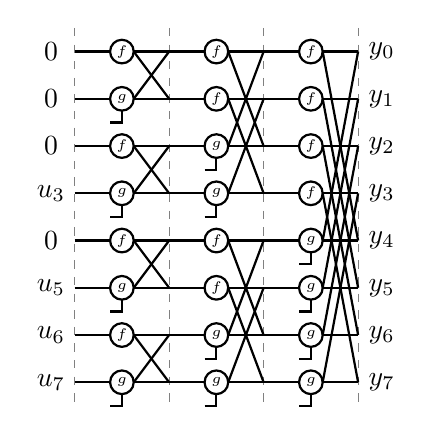
\begin{tikzpicture}[scale=.6, thick]

  \draw[very thin,gray,dashed] (1,.5) -- (1,-7.5);
  \draw[very thin,gray,dashed] (3,.5) -- (3,-7.5);
  \draw[very thin,gray,dashed] (5,.5) -- (5,-7.5);
  \draw[very thin,gray,dashed] (7,.5) -- (7,-7.5);

  %\node at (-.5,1) {layer};
  %\node at (1,1) {0};
  %\node at (3,1) {1};
  %\node at (5,1) {2};
  %\node at (7,1) {3};

  \node at (.5,0) {$0$};
  \node at (.5,-1) {$0$};
  \node at (.5,-2) {$0$};
  \node at (.5,-3) {$u_3$};
  \node at (.5,-4) {$0$};
  \node at (.5,-5) {$u_5$};
  \node at (.5,-6) {$u_6$};
  \node at (.5,-7) {$u_7$};

  \draw (1,0) -- ++(.75,0);
  \draw (2.25,0) -- ++(.75,0);
  \draw (1,-1) -- ++(.75,0);
  \draw (2.25,-1) -- ++(.75,0);

  \draw (2,0) circle [radius=.25] node {\tiny $f$};
  \draw (2,-1) circle [radius=.25] node {\tiny $g$};
  
  \draw (3,-1) -- ++(-.75,1);
  \draw (3,0) -- ++(-.75,-1);
  
  \draw (1.75,-1.5) -- ++(.25,0) -- ++(0,.25);

  \draw (1,-2) -- ++(.75,0);
  \draw (2.25,-2) -- ++(.75,0);
  \draw (1,-3) -- ++(.75,0);
  \draw (2.25,-3) -- ++(.75,0);

  \draw (2,-2) circle [radius=.25] node {\tiny $f$};
  \draw (2,-3) circle [radius=.25] node {\tiny $g$};
  
  \draw (3,-3) -- ++(-.75,1);
  \draw (3,-2) -- ++(-.75,-1);
  
  \draw (1.75,-3.5) -- ++(.25,0) -- ++(0,.25);

  \draw (1,-4) -- ++(.75,0);
  \draw (2.25,-4) -- ++(.75,0);
  \draw (1,-5) -- ++(.75,0);
  \draw (2.25,-5) -- ++(.75,0);

  \draw (2,-4) circle [radius=.25] node {\tiny $f$};
  \draw (2,-5) circle [radius=.25] node {\tiny $g$};
  
  \draw (3,-5) -- ++(-.75,1);
  \draw (3,-4) -- ++(-.75,-1);
  
  \draw (1.75,-5.5) -- ++(.25,0) -- ++(0,.25);

  \draw (1,-6) -- ++(.75,0);
  \draw (2.25,-6) -- ++(.75,0);
  \draw (1,-7) -- ++(.75,0);
  \draw (2.25,-7) -- ++(.75,0);

  \draw (2,-6) circle [radius=.25] node {\tiny $f$};
  \draw (2,-7) circle [radius=.25] node {\tiny $g$};
  
  \draw (3,-7) -- ++(-.75,1);
  \draw (3,-6) -- ++(-.75,-1);
  
  \draw (1.75,-7.5) -- ++(.25,0) -- ++(0,.25);

%-----

  \draw (3,0) -- ++(.75,0);
  \draw (4.25,0) -- ++(.75,0);
  \draw (3,-2) -- ++(.75,0);
  \draw (4.25,-2) -- ++(.75,0);

  \draw (4,0) circle [radius=.25] node {\tiny $f$};
  \draw (4,-2) circle [radius=.25] node {\tiny $g$};
  
  \draw (5,-2) -- ++(-.75,2);
  \draw (5,0) -- ++(-.75,-2);
  
  \draw (3.75,-2.5) -- ++(.25,0) -- ++(0,.25);

  \draw (3,-1) -- ++(.75,0);
  \draw (4.25,-1) -- ++(.75,0);
  \draw (3,-3) -- ++(.75,0);
  \draw (4.25,-3) -- ++(.75,0);

  \draw (4,-1) circle [radius=.25] node {\tiny $f$};
  \draw (4,-3) circle [radius=.25] node {\tiny $g$};
  
  \draw (5,-3) -- ++(-.75,2);
  \draw (5,-1) -- ++(-.75,-2);
  
  \draw (3.75,-3.5) -- ++(.25,0) -- ++(0,.25);

  \draw (3,-4) -- ++(.75,0);
  \draw (4.25,-4) -- ++(.75,0);
  \draw (3,-6) -- ++(.75,0);
  \draw (4.25,-6) -- ++(.75,0);

  \draw (4,-4) circle [radius=.25] node {\tiny $f$};
  \draw (4,-6) circle [radius=.25] node {\tiny $g$};
  
  \draw (5,-6) -- ++(-.75,2);
  \draw (5,-4) -- ++(-.75,-2);
  
  \draw (3.75,-6.5) -- ++(.25,0) -- ++(0,.25);

  \draw (3,-5) -- ++(.75,0);
  \draw (4.25,-5) -- ++(.75,0);
  \draw (3,-7) -- ++(.75,0);
  \draw (4.25,-7) -- ++(.75,0);

  \draw (4,-5) circle [radius=.25] node {\tiny $f$};
  \draw (4,-7) circle [radius=.25] node {\tiny $g$};
  
  \draw (5,-7) -- ++(-.75,2);
  \draw (5,-5) -- ++(-.75,-2);
  
  \draw (3.75,-7.5) -- ++(.25,0) -- ++(0,.25);

%-----

  \draw (5,0) -- ++(.75,0);
  \draw (6.25,0) -- ++(.75,0);
  \draw (5,-4) -- ++(.75,0);
  \draw (6.25,-4) -- ++(.75,0);

  \draw (6,0) circle [radius=.25] node {\tiny $f$};
  \draw (6,-4) circle [radius=.25] node {\tiny $g$};
  
  \draw (7,-4) -- ++(-.75,4);
  \draw (7,0) -- ++(-.75,-4);
  
  \draw (5.75,-4.5) -- ++(.25,0) -- ++(0,.25);

  \draw (5,-1) -- ++(.75,0);
  \draw (6.25,-1) -- ++(.75,0);
  \draw (5,-5) -- ++(.75,0);
  \draw (6.25,-5) -- ++(.75,0);

  \draw (6,-1) circle [radius=.25] node {\tiny $f$};
  \draw (6,-5) circle [radius=.25] node {\tiny $g$};
  
  \draw (7,-5) -- ++(-.75,4);
  \draw (7,-1) -- ++(-.75,-4);
  
  \draw (5.75,-5.5) -- ++(.25,0) -- ++(0,.25);

  \draw (5,-2) -- ++(.75,0);
  \draw (6.25,-2) -- ++(.75,0);
  \draw (5,-6) -- ++(.75,0);
  \draw (6.25,-6) -- ++(.75,0);

  \draw (6,-2) circle [radius=.25] node {\tiny $f$};
  \draw (6,-6) circle [radius=.25] node {\tiny $g$};
  
  \draw (7,-6) -- ++(-.75,4);
  \draw (7,-2) -- ++(-.75,-4);
  
  \draw (5.75,-6.5) -- ++(.25,0) -- ++(0,.25);

  \draw (5,-3) -- ++(.75,0);
  \draw (6.25,-3) -- ++(.75,0);
  \draw (5,-7) -- ++(.75,0);
  \draw (6.25,-7) -- ++(.75,0);

  \draw (6,-3) circle [radius=.25] node {\tiny $f$};
  \draw (6,-7) circle [radius=.25] node {\tiny $g$};
  
  \draw (7,-7) -- ++(-.75,4);
  \draw (7,-3) -- ++(-.75,-4);
  
  \draw (5.75,-7.5) -- ++(.25,0) -- ++(0,.25);

  \node at (7.5,0) {$y_0$};
  \node at (7.5,-1) {$y_1$};
  \node at (7.5,-2) {$y_2$};
  \node at (7.5,-3) {$y_3$};
  \node at (7.5,-4) {$y_4$};
  \node at (7.5,-5) {$y_5$};
  \node at (7.5,-6) {$y_6$};
  \node at (7.5,-7) {$y_7$};

\end{tikzpicture}